%!TEX root = ../dissertation.tex

\hypertarget{(chap:capitolo3)}{}
\chapter{Inquadramento delle attività di stage}
\section{Il progetto di stage}

Il progetto di stage, dopo l'evento \bit{StageIt}{stageit} ed alcune riunioni presso l'azienda, è stato studiato dettagliatamente e riportato nel documento "piano di lavoro", nello stesso sono riportati gli obiettivi e la pianificazione delle attività.

Questi esempi fanno riferimento a problematiche in ambito produttivo "Food and beverage", realizzando i moduli che si occupano della fatturazione degli alimenti, del loro inventario e dei clienti a cui corrispondono gli ordini. 
 Lo stage prevede la realizzazione di diversi moduli il cui sviluppo sarà incrementale in quanto ciascun modulo eredita struttura del modello e viste dai precedenti.
\newpage
Ogni modello odoo è identificato con un id (univoco) ed un nome che può essere individuato nelle impostazioni di odoo. Qui potremo individuare tutte le informazioni riguardo un dato modello, ad esempio: chi eredita, che campi contiene, autorizzazioni di accesso e viste. \\
Tutti questi dati permettono oggettivamente di valutare la corretta implementazione e creazione del modello.

\begin{figure}[H]
	\begin{center} 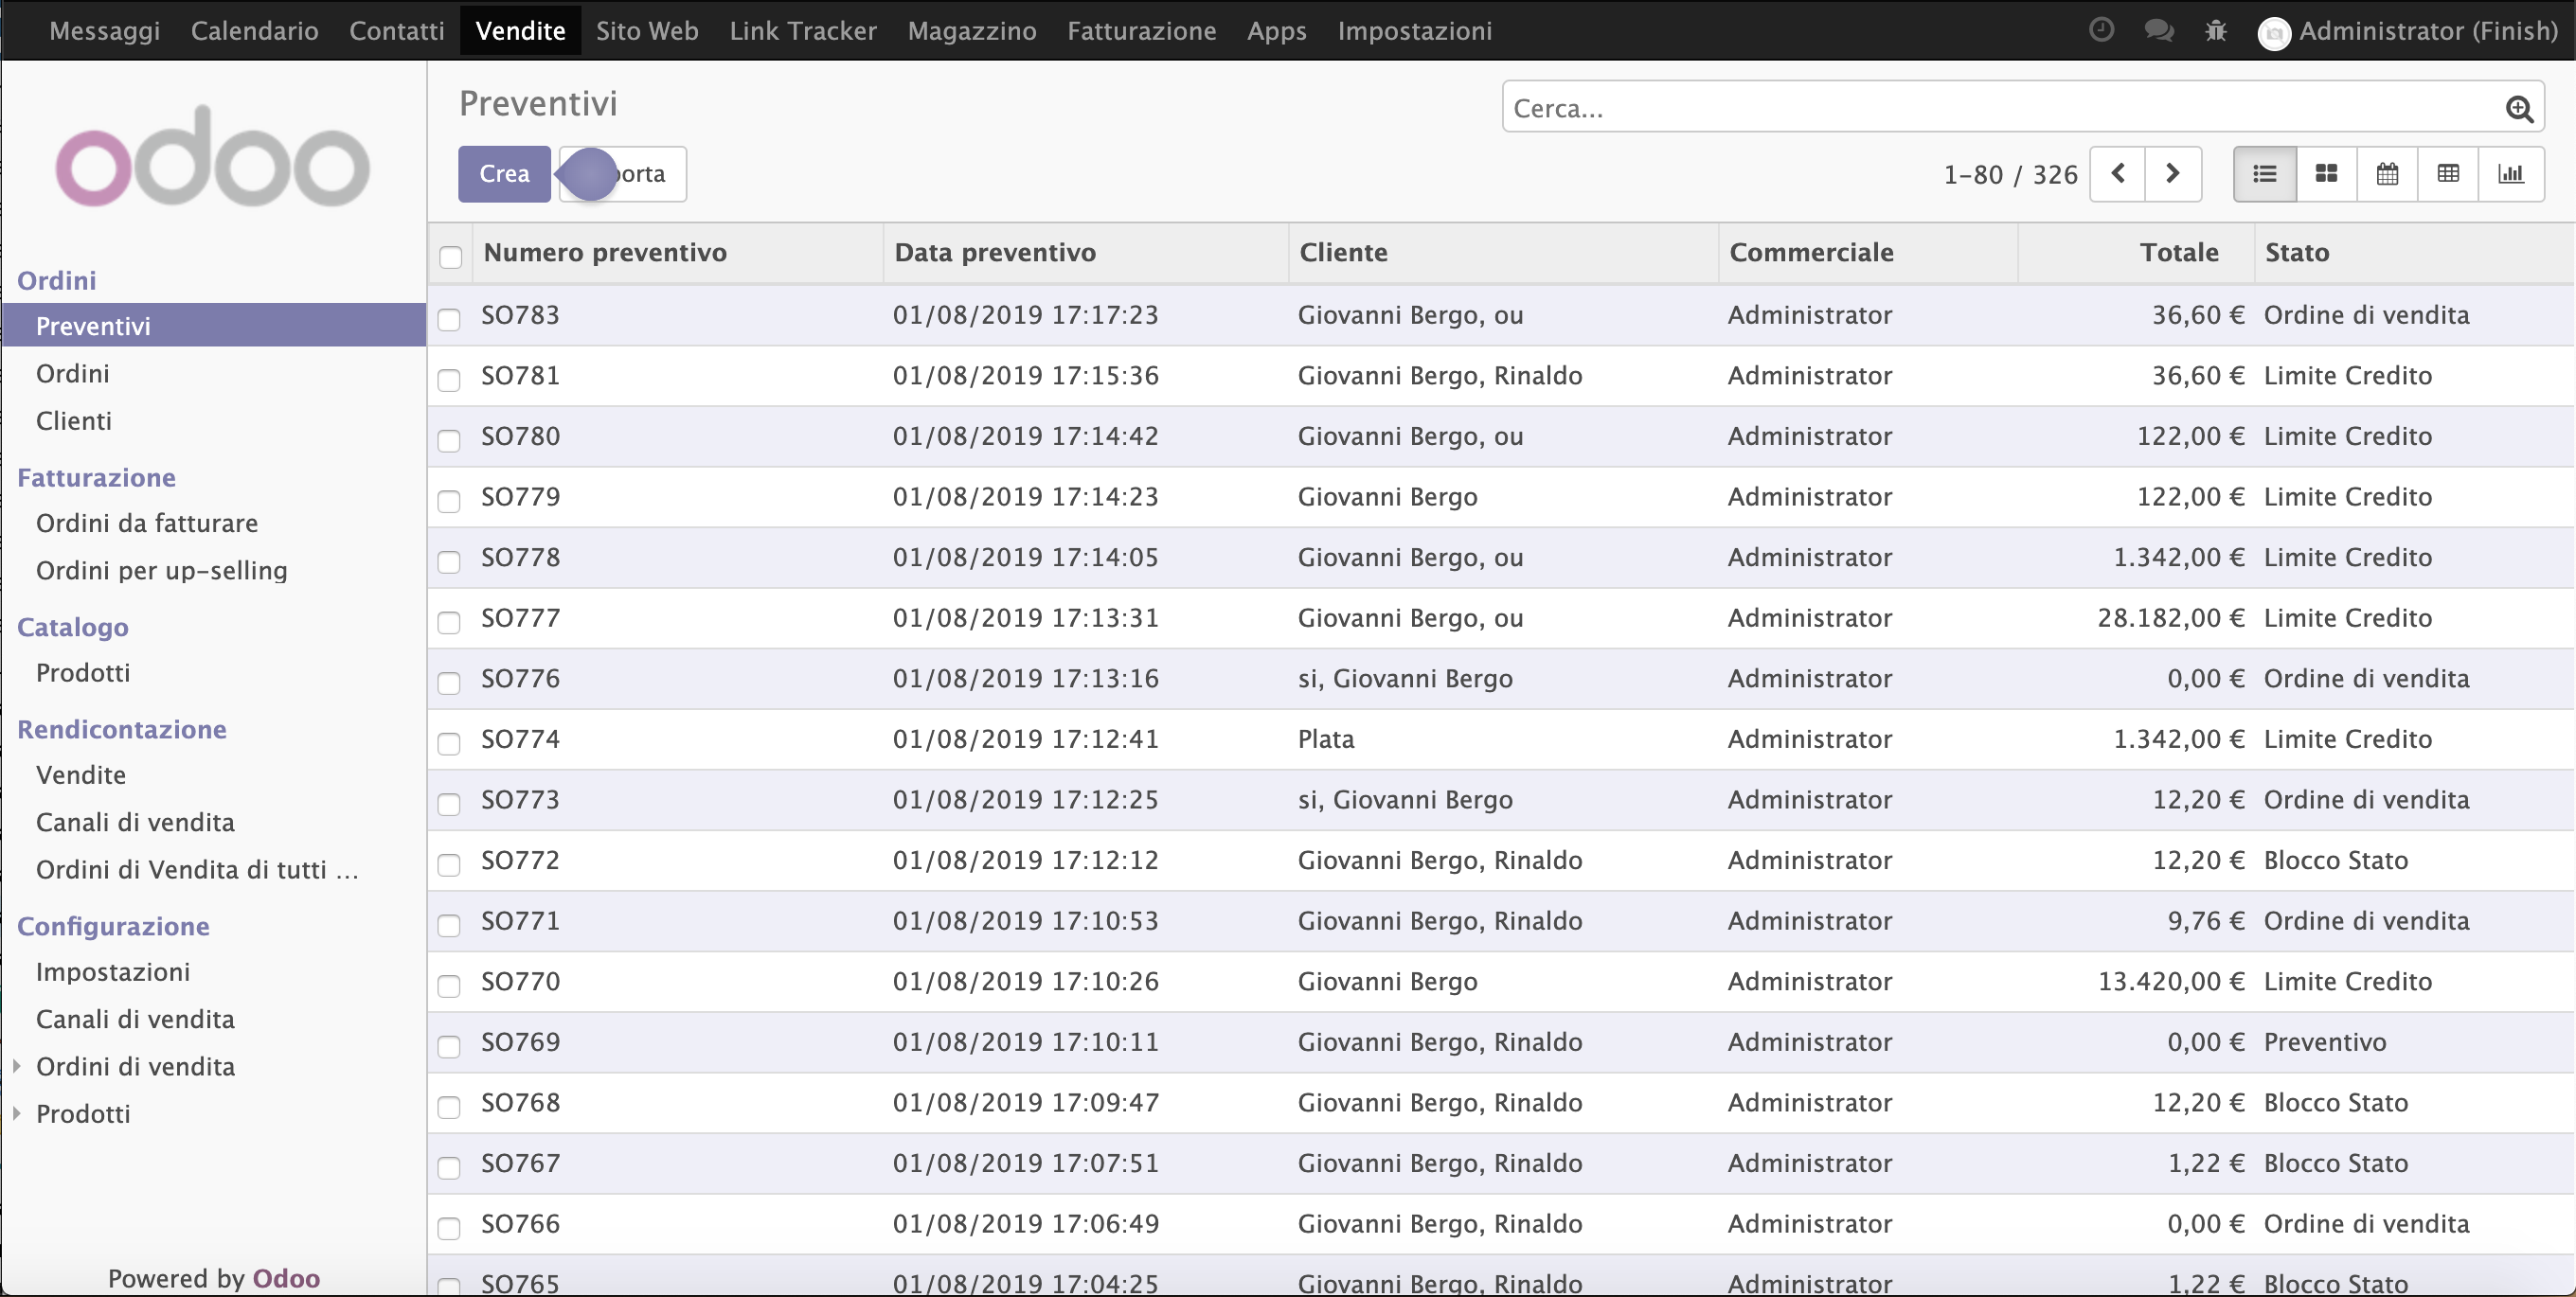
\includegraphics[scale=0.35]{figures/saleorder}
		\caption[Interfacciao vendite]{Interfaccia vendite Odoo}
		\label{fig:sale_order}
	\end{center}
\end{figure}

